\documentclass[fleqn, a4paper. 12pt]{jsarticle} 
\usepackage{amsmath,txfonts}
\usepackage{amssymb}
\usepackage{url}
\usepackage[margin=31mm]{geometry}
\usepackage[dvipdfmx]{graphicx}
\usepackage{listings,jvlisting}
\usepackage{fancyhdr}
\usepackage{lastpage}
\lstset{
  basicstyle={\ttfamily},
  identifierstyle={\small},
  commentstyle={\smallitshape},
  keywordstyle={\small\bfseries},
  ndkeywordstyle={\small},
  stringstyle={\small\ttfamily},
  frame={tb},
  breaklines=true,
  columns=[l]{fullflexible},
  numbers=left,
  xrightmargin=0zw,
  xleftmargin=3zw,
  numberstyle={\scriptsize},
  stepnumber=1,
  numbersep=1zw,
  lineskip=-0.5ex
}
\renewcommand{\lstlistingname}{プログラム}

% header
\pagestyle{fancy}
\fancyhf{}
\rhead{2024-05}
\lhead{谷 知拓 - Tomohiro Tani}
\cfoot{\thepage\ / \pageref{LastPage}}


\begin{document}
  \begin{titlepage}
    \begin{center}
      {\Huge 2024年度\\応用プログラミング実験}
      
      \vspace{4cm}
      {\Huge 第4回\\マルチメディア情報検索\\
        実験レポート\\
      }
      \vspace{4cm}
      {\large 学修番号: 22140026\\谷 知拓 - Tomohiro Tani\footnote{東京都立大学 システムデザイン学部 情報科学科 \\ mail@taniii.com} \\}
      \vspace{0.5cm}
      {\large
        レポート提出日 : 2024-05-09 \\
      }
    \end{center}
  \end{titlepage}
  
  \section{はじめに}
    本書では,『応用プログラミング実験』第4回の実施報告を行う.\\
    部分空間法を用いて手書きの数字の認識を行う.\\

  \section{実験環境}

    実験環境は以下の通りである.

    \begin{itemize}
      \item OS\footnote{Operating System}: macOS Ventura 13.4.1
      \item CPU\footnote{Central Processing Unit}: Apple M2 arm64\footnotemark[7]
      \item メインメモリ・ビデオメモリ共通: 16GBユニファイドメモリ\footnotemark[7]
      \footnotetext[7]{https://www.apple.com/jp/macbook-air-13-and-15-m2/specs/}
      \item 実行環境 (matlab): matlab R2023b (23.2.0.2380103) 64-bit (maca64)
    \end{itemize}

  \section{実験の概要}

    本実験では,部分空間法を用いて手書きの数字の認識を行う.

    手書きの数字のデータセットを用いて,部分空間法を用いて手書きの数字の認識を行う.

    また,部分空間法を用いて手書きの数字の認識を行う際に,どのような手法を用いるか,また,その手法を用いることでどのような効果があるかを考察する.

  \section{部分空間法の原理}

    部分空間法は, パターン認識において広く用いられる手法であり,高次元データの持つ構造をより低次元の空間に射影し,その射影された空間でのデータの特性を利用して識別を行う手法である.

    この手法を用いて,データの次元を削減することで,様々なパターン変動 (認識対象のパターンが様々な要因により変化すること) を,小さい辞書で表現することができ,高速かつ高精度な認識が可能となる.

    部分空間法を用いたパターン認識の基本的な流れは,まず学習段階において,クラスごとに,エントロピーが最小化されるような部分空間 (より低次元な空間) を見つける.

    そして,識別段階において,データをその部分空間に射影し,射影されたデータの特性を利用して識別を行う.

    以下では,具体的な手法について説明する.



    \subsection{学習}

        学習段階においては,クラスごとに,エントロピーが最小化されるような部分空間を見つける.
    
        式 \ref{eq:1} で表されるエントロピーが最小となるような,部分空間軸を求める.

        \begin{equation}
            \min _{\boldsymbol{u}_i}-\sum_{i=1}^d p\left(\boldsymbol{u}_i\right) \log p\left(\boldsymbol{u}_i\right)
            \label{eq:1}
        \end{equation}

        ただし,$p\left(\boldsymbol{u}_i\right)$ は,部分空間軸 $\boldsymbol{u}_i$ におけるデータの分布を表す確率密度関数である.

        \quad

        ここで,データから最適な部分空間軸 (部分空間の基底ベクトル) を求めるために,主成分分析 (PCA) や線形判別分析 (LDA) を用いる方法がある.
        
        主成分分析において,最も分散が大きい方向を求める場合や,線形判別分析において,クラス間分散を最大化しつつクラス内分散を最小化する方向を見つける場合に,
        \textbf{制約付き最適化問題} を解く必要があり,これに \textbf{ラグランジュの未定乗数法} を用いることがある.

        \quad

        ラグランジュの未定乗数法は,以下のように解くことができる.

        仮に,以下のような制約付き最適化問題を考える.

        \begin{quote}
            制約条件
            $g(\boldsymbol{x})=0$
            のもとで関数
            $f(\boldsymbol{x})$ 
            の極地を求めよ
        \end{quote}

        \quad

        まず,ラグランジュ関数を以下のように定義する.

        \begin{equation}
            L(\boldsymbol{x}, \lambda)=f(\boldsymbol{x})+\lambda g(\boldsymbol{x})
        \end{equation}

        このラグランジュ関数を最小化するために,以下のような方程式を解く.

        \begin{equation}
            \frac{\partial}{\partial \boldsymbol{x}} L=\nabla f-\lambda \nabla g=\mathbf{0}, \frac{\partial L}{\partial \lambda}=0
        \end{equation}

        この方程式を解くことで,制約条件のもとでの関数の極値を求めることができる.

        \quad

        部分空間法では,$\boldsymbol{u}^{\top} \boldsymbol{u}=1$ を制約条件として,
        $\boldsymbol{u}^{\top} \mathbf{A} \boldsymbol{u}$ の最大値を求める問題を解く必要があることが頻出である.

        \begin{equation}
            \begin{gathered}
            \max _{\boldsymbol{u}} \boldsymbol{u}^{\top} \mathbf{A} \boldsymbol{u} \\
            \text { s.t. } \boldsymbol{u}^{\top} \boldsymbol{u}-1=0
            \end{gathered}
        \end{equation}

        ただし,$\mathbf{A}$ は半正定値対称行列である.

        \quad

        このような問題を解くために,ラグランジュの未定乗数法を用いることがある.

        ラグランジュ乗数 $\lambda$ を導入し,ラグランジュ関数を以下のように定義する.

        \begin{equation}
            L(\boldsymbol{u}, \lambda)=\boldsymbol{u}^{\top} \mathbf{A} \boldsymbol{u}+\lambda\left(\boldsymbol{u}^{\top} \boldsymbol{u}-1\right)
        \end{equation}

        制約条件のもとで,関数が極値を取る点は次式を満たす.

        \begin{equation}
            \partial L / \partial \boldsymbol{u}=\mathbf{0}, \partial L / \partial \lambda=0
        \end{equation}

        $\partial L / \partial \boldsymbol{u}=2 \mathbf{A} \boldsymbol{u}-2 \lambda \boldsymbol{u}=\mathbf{0}$
        より,$\mathbf{A} \boldsymbol{u}=\lambda \boldsymbol{u}$ が成り立つ.

    \subsection{識別}

        続いて,識別段階においては,データを学習によって得られた部分空間に射影し,射影されたデータの特性を利用して,クラス分けを行う.

        \quad

        識別においては,以下のような問題設定を考える.

        \begin{quote}
            \begin{enumerate}
                \item 総数 $n$ 個の $d$ 次元訓練パターン $x_i$ が与えられており,それらが $C$ 個のクラスのいずれか 1 つに分類されている.
                \item クラス $j$ に属する訓練パターンを良く近似することのできる部分空間を張る正規直交ベクトルの行列を $\mathbf{U}_j$ とする.
            \end{enumerate}
        \end{quote}

        このとき,未知パターン $x$ が与えられたとき,属するクラスを求めるための,部分空間法の識別則は以下のように定義できる.

        \begin{equation}
            \max _{j=1, \ldots, C}\left\{\left\|\mathbf{U}_j^{\top} \boldsymbol{x}\right\|\right\}=\left\|\mathbf{U}_k^{\top} \boldsymbol{x}\right\| \Rightarrow \boldsymbol{x} \in \text { class } k
        \end{equation}

        これは,未知パターン $x$ を各クラスの部分空間に射影し,射影されたデータのノルムが最大となるクラスに分類するということを意味している.

        \quad

        部分空間法よりシンプルな識別則として,最小距離法が考えられるが,これは,$d_j^2 = \|x\|^2 - \|U_j^T x\|^2$ 
        が最小となるクラスに分類するというものである.

        ただし,$d_j$ は,未知パターン $x$ とクラス $j$ の部分空間との距離を表す.

        \quad

        ここで,$\|x\|^2$ は,クラスに関わらず共通であるため,$\|U_j^T x\|^2$ が最大となるクラスを探せば良い.

        したがって,最小距離法による識別則と,部分空間法による識別則は,矛盾しない.

        このようにして,部分空間法を用いて,未知パターンをクラス分けすることができる.

  \section{実験結果}

    実験結果は以下の通りである.

    図 \ref{fig:1} は,次元 $r = 1, \dots, 20$ と認識率の関係をグラフにしたものである.

    \begin{figure}
      \centering
      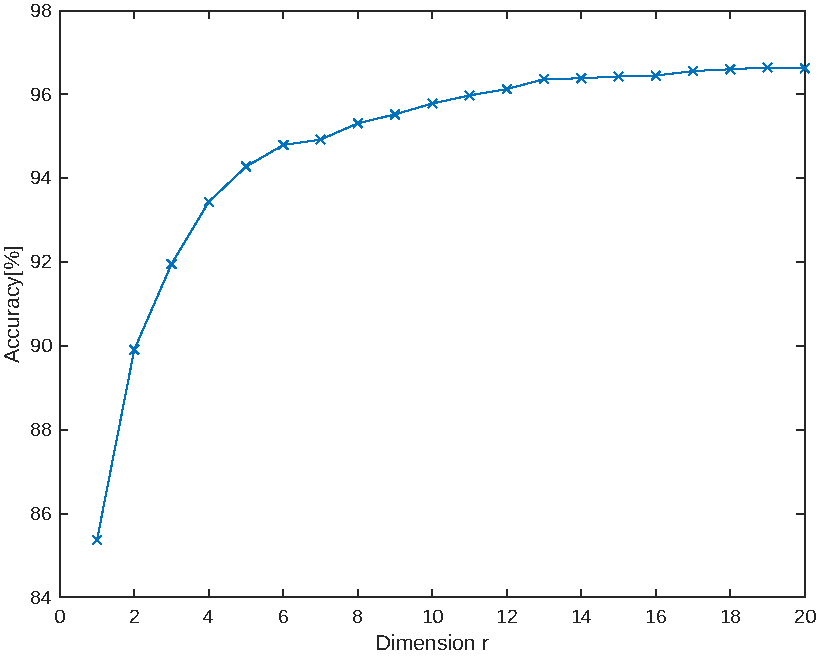
\includegraphics[width=1\textwidth]{fig_0.pdf}
      \caption{次元 $(r = 1, \dots, 20)$ と認識率の関係}
      \label{fig:1}
    \end{figure}

  \section{付録}

    作成したソースコードを以下に示す.

    \begin{lstlisting}
      // global.h
      #include <stdio.h>
      #include <stdlib.h>
      #include <string.h>
      #include <ctype.h>

      #define BSIZE 128
      #define NONE  -1
      #define EOS   '\0'

      #define NUM   256
      #define DIV   257
      #define MOD   258
      #define ID    259
      #define DONE  260

      #define ASSIGN 261

      #define WHILE 262
      #define DO 263
      #define BEGIN 263
      #define END 264

      int tokenval;
      int lineno;

      struct entry {
        char *lexptr;
        int token;
      };

      struct entry symtable[];

      int lexan();
      void parse();
      void stmt();
      void stmt_list();
      void expr();
      void term();
      void factor();
      void cond();
      void match(int);
      void emit(int, int);
      int lookup(char[]);
      int insert(char[], int);
      void init();
      void error(char*);


      // lexer.c
      char lexbuf[BSIZE];
      int lineno = 1;
      int tokenval = NONE;

      int lexan()
      {
        int t;
        while(1) {
          t = getchar();
          if (t == ' ' || t == '\t')
            ;
          else if ( t == '\n')
            lineno = lineno + 1;
          else if (t == ':') {
            if (getchar() == '=') {
              return ASSIGN;
            }
          }
          else if (isdigit(t)) {
            ungetc(t, stdin);
            scanf("%d", &tokenval);    // for gcc
            //scanf_s("%d", &tokenval);    // for Visual Studio
            return NUM;
          }
          else if (isalpha(t)) {
            int p,b = 0;
            while (isalnum(t)) {
              lexbuf[b] = t;
              t = getchar();
              b = b + 1;
              if (b >= BSIZE)
                error("compiler error");
            }
            lexbuf[b] = EOS;
            if (t !=EOF)
              ungetc(t, stdin);
            p = lookup(lexbuf);
            if (p == 0)
              p = insert(lexbuf, ID);
            tokenval = p;
            return symtable[p].token;
          }
          else if (t == EOF)
            return DONE;
          else {
            tokenval = NONE;
            return t;
          }
        }
      }


      // parser.c
      int lookahead;

      void parse()
      {
        // 1 トークン分読んで型が代入される
        lookahead = lexan();
        while (lookahead != DONE) {
          stmt(); match(';');
        }
      }

      // statement
      void stmt()
      {
        // 文の解析を行う
        // それぞれ 1 つ目の文字に引っかかったら次の文字を読み込む
        switch (lookahead) {
        case ID: // 代入文の翻訳
          printf("lvalue\t"); // "lvalue" は左辺値のこと
          emit(ID, tokenval); // 出力関数を呼び出し
          match(lookahead); // 先読み
          if (lookahead == ASSIGN) {
            match(lookahead); // 先読み
            // 代入文の右辺の式を解析
            expr();
            printf(":=\n");
          }
          break;
        
        case WHILE: // while 文の翻訳
          match(WHILE);
          printf("label\ttest\n");
          cond();
          printf("gofalse\tout\n");
          match(DO);
          stmt();
          printf("goto\ttest\n");
          printf("label\tout\n");
          break;

        case BEGIN:
          match(BEGIN);
          stmt();
          while (lookahead != END) {
            match(lookahead); // 先読み
            stmt();
          }
          match(END);
          break;

        default:
          break;
        }
      }

      void expr()
      {
        int t;
        term();
        while(1)
          switch (lookahead) {
          case '+': case '-':
            t = lookahead;
            match(lookahead); term(); emit(t, NONE);
            continue;
          default:
            return;
          }
      }

      void term()
      {
        int t;
        factor();
        while(1)
          switch (lookahead) {
          case '*': case '/': case DIV: case MOD:
            t = lookahead;
            match(lookahead);
            factor();
            emit(t, NONE);
            continue;
          default:
            return;
          }
      }

      void factor()
      {
        switch(lookahead) {
          case '(':
            match('('); expr(); match(')'); break;
          case NUM:
            printf("push\t");
            emit(NUM, tokenval); match(NUM); break;
          case ID:
            printf("rvalue\t");
            emit(ID, tokenval);
            match(ID);
            break;
          default:
            error("syntax error"); break;
        }
      }

      void cond()
      {
        int t;
        expr();
        
        switch (lookahead)
        {
        case '<': case '>': case '=':
          t = lookahead;
          match(lookahead);
          expr();
          emit(t, NONE);
          break;
        default:
          break;
        }
        return;
      }

      // 現在の先読みトークンが t と一致するかどうかを確認し, 次の先読みトークンを読み込む
      void match(t)
        int t;
      {
        if (lookahead == t)
          lookahead = lexan();
        else error("syntax error");
      }


      // emitter.c
      void emit(t, tval)
        int t, tval;
      {
        switch(t) {
          case '+': case '-': case '*': case '/': case '<': case '>': case '=':
            printf("%c\n", t); break;
          case DIV:
            printf("DIV\n"); break;
          case MOD:
            printf("MOD\n"); break;
          case NUM:
            printf("%d\n", tval); break;
          case ID:
            printf("%s\n", symtable[tval].lexptr); break;
          default:
            printf("token %d, tokenval %d\n", t, tval); break;
        }
      }


      // symbol.c
      #define STRMAX	999
      #define SYMMAX	100

      char lexemes[STRMAX];
      int lastchar = -1;
      struct entry symtable[SYMMAX];
      int lastentry = 0;

      int lookup(s)
        char s[];
      {
        int p;
        for (p = lastentry; p > 0; p = p -1)
          if (strcmp(symtable[p].lexptr, s) == 0)
            return p;
        return 0;
      }

      int insert(s, tok)
        char s[];
        int tok;
      {
        int len;
        len = strlen(s);
        if (lastentry +1 >= SYMMAX)
          error("symbol table full");
        if (lastchar + len +1 >= STRMAX)
          error("lexemes array full");
        lastentry = lastentry +1;
        symtable[lastentry].token = tok;
        symtable[lastentry].lexptr = &lexemes[lastchar + 1];
        lastchar = lastchar + len + 1;
        strcpy(symtable[lastentry].lexptr, s);
        return lastentry;
      }


      // init.c
      struct entry keywords[] = {
        "div", DIV,
        "mod", MOD,
        "while", WHILE,
        "do", DO,
        "begin", BEGIN,
        "end", END,
        0, 0
      };

      void init()
      {
        struct entry *p;
        for (p = keywords; p -> token; p++)
          insert(p -> lexptr, p -> token);
      }


      // error.c
      void error(m)
        char *m;
      {
        fprintf(stderr, "line %d: %s\n", lineno, m);
        exit(1);
      }


      // main.c
      void main()
      {
        init();
        parse();
        exit(0);
      }

    \end{lstlisting}

\end{document}